\chapter{Hasil dan Pembahasan}

\section {Lingkungan Eksperimen}

Pengumpulan \textit{dataset} dilakukan pada lingkungan komputasi dan penyimpanan sebagai berikut:

\begin{enumerate}[label=\Alph{enumi}.,topsep=0pt,itemsep=0pt,parsep=0pt]
    \item Klien Pelatihan
        \begin{itemize}[itemsep=0pt, parsep=0pt]
            \item Prosesor: Intel Xeon Silver 4210R (10 \textit{Cores} @ 2.40GHz, 64-bit)
            \item RAM: 80 GB
            \item GPU: Tidak ada
            \item Disk Lokal: 145 GB NVMe SSD
            \item Sistem Operasi: Ubuntu 18.04
            \item Versi Kernel: 5.4.0-150-generic
        \end{itemize}

    \item \textit{Server} Penyimpanan NFS
        \begin{itemize}[itemsep=0pt, parsep=0pt]
            \item Prosesor: Intel Xeon Silver 4110 (16 \textit{Cores} @ 2.10 GH, 64-bit)
            \item RAM: 32 GB
            \item Penyimpanan \textit{Dataset}: RAID 5 dari 3x 6.4 TB
            \item Versi NFS: NFSv4.1
        \end{itemize}
    
    \item Jaringan
        \begin{itemize}[itemsep=0pt, parsep=0pt]
            \item Terhubung melalui ethernet dengan rata-rata \textit{bandwidth} 11,4 Mbps dan rata-rata \textit{Return Trip Time} 0,294 ms
        \end{itemize}

    \item Perangkat Lunak
        \begin{itemize}[itemsep=0pt, parsep=0pt]
            \item Python: 3.8.20
            \item PyTorch: 2.4.1
            \item bpftrace: v0.22.1
        \end{itemize}
\end{enumerate}

\section{Pelaksanaan Eksperimen dan Pengumpulan Data}

\begin{figure}[t]
    \centering
    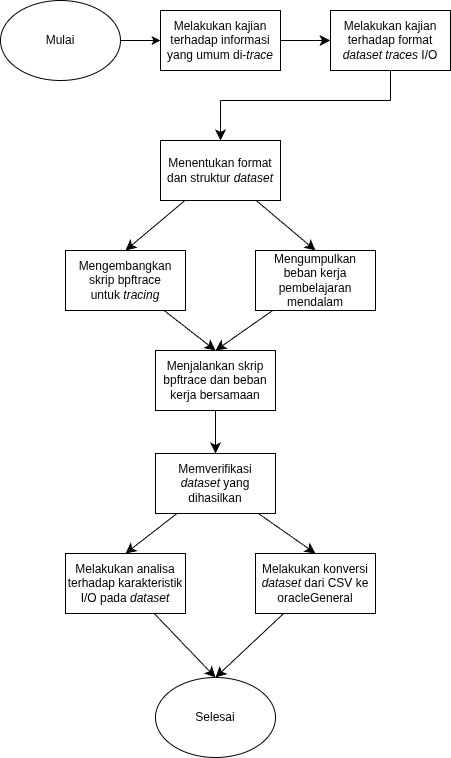
\includegraphics[width=0.6\textwidth]{FlowchartPengerjaan.png}
    \caption{Alur Pengembangan \textit{Dataset}}
    \label{fig:FlowchartPengerjaan}
\end{figure}

Pengembangan \textit{dataset trace} I/O NFS merupakan tujuan utama dari tugas akhir ini. Proses pengembangan \textit{dataset} dilakukan secara sistematis mengikuti alur kerja yang telah diilustraikan pada Gambar \ref{fig:FlowchartPengerjaan}. Sebelum eksekusi, semua komponen telah disiapkan sesuai dengan pembahasan pada Bab III. Sebagai ringkasan, konfigurasi yang digunakan adalah sebagai berikut:
\begin{enumerate}[itemsep=0pt, parsep=0pt]
    \item Informasi pada \textit{Dataset}: Tiga informasi utama yang di-\textit{trace} untuk setiap akses I/O NFS, yaitu \texttt{timestamp}, \texttt{obj\_id}, dan \texttt{obj\_size}, dengan detail seperti yang dirangkum pada Tabel \ref{tab:trace_format}.
    \item Format \textit{Dataset}: \textit{Dataset} final akan disajikan dalam dua format: CSV untuk kemudahan analisis dan oracleGeneral untuk kompatibilitas dengan \textit{simulator} \texttt{libCacheSim}.
    \item \textit{Tracer}: Sebuah skrip \texttt{bpftrace} kustom (dijelaskan pada Subbab \ref{sec:pengembangan_tracer}) digunakan sebagai \textit{tracer}.
    \item Beban Kerja: Beban kerja yang di-\textit{trace} adalah proses iterasi \textit{dataset} pada skenario klasifikasi gambar dengan berbagai strategi \textit{shuffling} (dijelaskan pada Subbab \ref{sec:bebankerja}).
\end{enumerate}

\begin{table}[t]
    \centering
    \caption{Struktur Informasi pada Setiap Entri \textit{Trace}}
    \label{tab:trace_format}
    \begin{tabular}{|l|p{0.6\textwidth}|}
        \hline
        \textbf{Kolom} & \textbf{Deskripsi} \\
        \hline
        \texttt{timestamp} & Waktu relatif saat permintaan I/O terjadi, diukur dalam satuan nanodetik sejak sistem dinyalakan. \\
        \hline
        \texttt{obj\_id}    & ID unik dalam format \textit{integer} yang merepresentasikan setiap berkas yang diakses. \\
        \hline
        \texttt{obj\_size}  & Ukuran total dari berkas yang diakses dalam satuan byte. \\
        \hline
    \end{tabular}
\end{table}

Proses perekaman \textit{trace} dilakukan dengan menjalankan skrip \texttt{bpftrace} dan beban kerja pembelajaran mendalam secara sinkron untuk setiap konfigurasi eksperimen. Keluaran standar dari \texttt{bpftrace}, yang berisi data \textit{trace} baris per baris, dialihkan dan disimpan langsung ke dalam sebuah berkas dengan format \texttt{.csv} menggunakan utilitas \texttt{tee} pada terminal Linux. Pendekatan ini memastikan perekaman data terjadi secara waktu-nyata dengan \textit{overhead} minimal pada proses yang sedang diamati.

Setelah proses perekaman untuk setiap konfigurasi selesai, dilakukan tahap verifikasi data. Proses ini krusial untuk memastikan bahwa \textit{trace} yang dihasilkan bebas dari anomali, lengkap, dan secara akurat merefleksikan aktivitas I/O yang terjadi. Proses validasi dilakukan dengan beberapa pendekatan berikut:
\begin{enumerate}
    \item Konsistensi Waktu: Memastikan nilai pada kolom \texttt{timestamp} selalu terurut menaik.
    \item Konsistensi Ukuran: Memastikan setiap \texttt{obj\_id} yang sama selalu memiliki nilai \texttt{obj\_size} yang identik, karena operasi hanya bersifat baca.
    \item Konsistensi ID: Memastikan setiap \texttt{obj\_id} secara konsisten merujuk pada satu \texttt{obj\_name} yang sama. Untuk tujuan ini, nama berkas juga direkam dalam \textit{trace} mentah namun kemudian dihapus dari \textit{dataset} final untuk menjaga format tetap ringkas.
\end{enumerate}


Setelah sebuah berkas \textit{trace} dinyatakan valid, dua lanxgkah akhir dilakukan. Pertama, untuk tujuan kompatibilitas dengan \textit{simulator} \texttt{libCacheSim}, berkas CSV dikonversi ke format \texttt{oracleGeneral} menggunakan kakas yang disediakan oleh \texttt{libCacheSim}. Kedua, dilakukan analisis karakteristik I/O pada \textit{dataset} CSV menggunakan pendekatan yang telah dijelaskan pada Subbab \ref{sec:metopenkarakteristik}. Dari hasil pengumpulan data ini, dihasilkan serangkaian \textit{dataset trace} I/O NFS yang dirangkum pada Tabel \ref{tab:trace_dataset}.

\begin{table}[t]
    \centering
    \caption{Deskripsi Berkas pada Dataset yang Dihasilkan}
    \label{tab:trace_dataset}
    \begin{tabular}{|l|l|c|c|c|l|}
        \hline
        \thead{\bfseries Nama Berkas} & \thead{\bfseries Dataset} & \thead{\bfseries Kehadiran\\ \bfseries Data Validasi} & \thead{\bfseries Jumlah\\ \bfseries Epoch} & \thead{\bfseries Jumlah\\ \bfseries Worker} & \thead{\bfseries Variasi Shuffling} \\
        \hline
        
        \texttt{\makecell[t]{firerisk\_val\\\_global\_0w}}    & FireRisk & Ada   & 100 & 0  & \textit{Global Shuffling} \\
        \hline
        \texttt{\makecell[t]{firerisk\_val\\\_global\_16w}}   & FireRisk & Ada   & 100 & 16 & \textit{Global Shuffling} \\
        \hline
        \texttt{\makecell[t]{firerisk\\\_global\_0w}}       & FireRisk & Tidak & 100 & 0  & \textit{Global Shuffling} \\
        \hline
        \texttt{\makecell[t]{firerisk\\\_global\_16w}}      & FireRisk & Tidak & 100 & 16 & \textit{Global Shuffling} \\
        \hline
        
        \texttt{\makecell[t]{firerisk\_val\\\_buffer1000\_0w}}  & FireRisk & Ada   & 100 & 0  & \makecell[t]{\textit{Buffered Shuffling}\\(\textit{buffer size} 1000)} \\
        \hline
        \texttt{\makecell[t]{firerisk\_val\\\_buffer1000\_16w}} & FireRisk & Ada   & 100 & 16 & \makecell[t]{\textit{Buffered Shuffling}\\(\textit{buffer size} 1000)} \\
        \hline
        \texttt{\makecell[t]{firerisk\\\_buffer1000\_0w}}      & FireRisk & Tidak & 100 & 0  & \makecell[t]{\textit{Buffered Shuffling}\\(\textit{buffer size} 1000)} \\
        \hline
        \texttt{\makecell[t]{firerisk\\\_buffer1000\_16w}}     & FireRisk & Tidak & 100 & 16 & \makecell[t]{\textit{Buffered Shuffling}\\(\textit{buffer size} 1000)} \\
        \hline

        \texttt{\makecell[t]{firerisk\_val\\\_bundle1000\_0w}}  & FireRisk & Ada   & 100 & 0  & \makecell[t]{\textit{Bundle Shuffling}\\(\textit{bundle size} 1000)} \\
        \hline
        \texttt{\makecell[t]{firerisk\_val\\\_bundle1000\_16w}} & FireRisk & Ada   & 100 & 16 & \makecell[t]{\textit{Bundle Shuffling}\\(\textit{bundle size} 1000)} \\
        \hline
        \texttt{\makecell[t]{firerisk\\\_bundle1000\_0w}}      & FireRisk & Tidak & 100 & 0  & \makecell[t]{\textit{Bundle Shuffling}\\(\textit{bundle size} 1000)} \\
        \hline
        \texttt{\makecell[t]{firerisk\\\_bundle1000\_16w}}     & FireRisk & Tidak & 100 & 16 & \makecell[t]{\textit{Bundle Shuffling}\\(\textit{bundle size} 1000)} \\
        \hline
    \end{tabular}
\end{table}

\section{Karakteristik \textit{Temporal Locality}}
\blindtext

\section{Hasil Pengujian}
\blindtext

\section{Pembahasan}
\blindtext